\subsection{Incremental Rejection}
Incremental rejection preserves every K12 and Full-203 decision, selected rank, and selected cost across all 432 matched inputs. Repeating the closed-loop matrix also reproduces all 480 outcomes, 27,771 trajectory records, and 27,291 planning decisions exactly; only computation and rejection accounting change. It substantially reduces the work needed to obtain those decisions. Mean continuation integration falls from 20,605 to 6,210 steps for Cost-12, from 21,054 to 2,654 for Diverse-12, and from 81,388 to 13,698 for Full-203. These reductions are 69.86\%, 87.39\%, and 83.17\%, respectively. Figure~\ref{fig:incremental} compares both validators.

The reduction changes the work-limited search. At $W=3{,}600$, incremental cost ordering finds 204 of the 335 reference witnesses, whereas incremental diversity finds 269: recall increases from 60.90\% to 80.30\%. The paired difference is 19.40 percentage points with a 95\% map interval of [6.63,34.66]. At $W=10{,}800$, the corresponding counts are 227 and 317, or 67.76\% and 94.63\%. The difference is 26.87 percentage points [15.00,40.46], with 90 inputs found only by diversity and none found only by cost ordering.

With failed rollouts removed early, the 10,800-step diversity search reaches the same 317 witnesses as the 12-candidate diversity search. This result connects the scheduling and validation components: dispersed terminal endpoints provide useful alternatives only when the validator can reach them within its work allowance. The complete-rollout ablation does not exhibit a diversity advantage at these work limits.

Incremental Diverse-12 has median, P95, and P99 planning times of 2.89, 4.62, and 4.72 ms. Incremental Cost-12 gives 2.74, 6.68, and 6.88 ms, while Full-203 gives 2.74, 11.71, and 12.38 ms. The diversity schedule has a slightly larger median than cost ordering but a shorter upper tail. These timings come from separate runs of the two validator implementations; the exact integration counters provide the direct measure of eliminated numerical work.

\begin{figure*}[!t]
\centering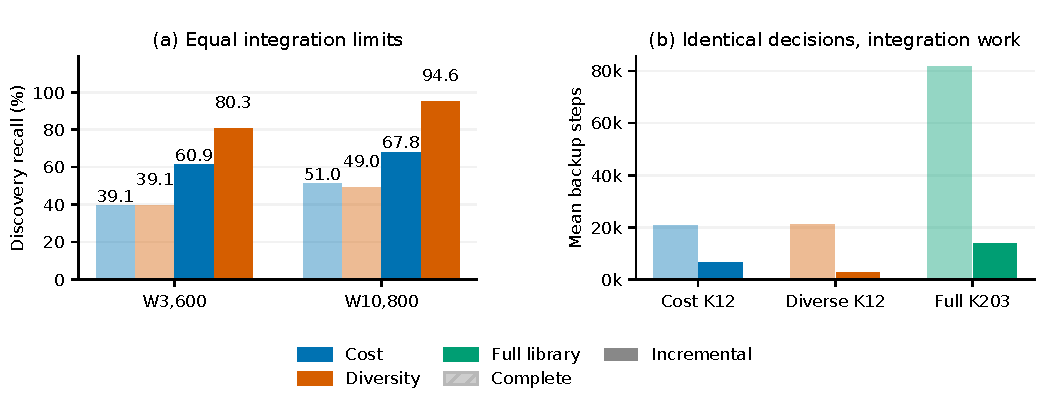
\includegraphics[width=\textwidth]{figures/incremental.pdf}
\caption{Effect of incremental rejection on the same matched inputs. Work-budget comparisons use identical upper limits; consumed work can be smaller after early success. The complete-rollout results are retained to isolate the effect of ending a continuation at its first violated constraint.}
\label{fig:incremental}
\end{figure*}
